%!TEX root = ../../main.tex

\begin{figure}
\begin{center}
\caption{
    Dependency Graph of the Morpheus GraphQL Packages
    \label{fig:dependency-graph}
    }
\footnotesize
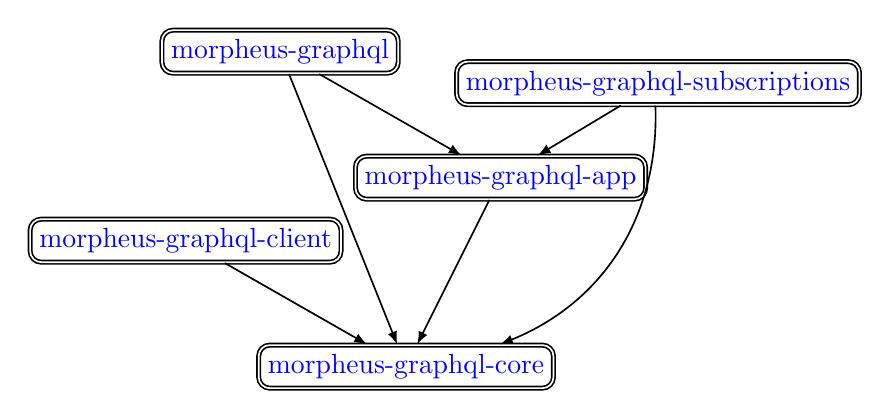
\begin{tikzpicture}[
        scale=.4,
        auto=left,
        -latex ,
        auto ,
        node distance =2 cm and 2cm ,
        % on grid ,
        semithick ,
        package/.style ={ fill=red!20,draw,double,rounded corners ,top color =white ,draw , text=blue , minimum width =1 cm},
    ] 
    \node[package] (core) at (10,0) {morpheus-graphql-core};
    \node[package] (client) at (3,4)  {morpheus-graphql-client};
    \node[package] (app) at (13,6)  {morpheus-graphql-app};
    \node[package] (server) at (6,10)  {morpheus-graphql};
    \node[package] (subs) at (18,9) {morpheus-graphql-subscriptions};
  
    \path (client) edge (core);
    \path (app)  edge (core);
    \path (server)  edge  (core);
    \path (server)  edge  (app);
    \path (subs)  edge  (app);
    \path 
        (subs) 
            edge [bend left =35] 
        (core);  

\end{tikzpicture}
\end{center}
\end{figure}
